\documentclass[12pt]{article}

\usepackage[margin=1in]{geometry} 
\usepackage{amsmath}
\usepackage{tcolorbox}
\usepackage{amssymb}
\usepackage{amsthm}
\usepackage{lastpage}
\usepackage{fancyhdr}
\usepackage{accents}

\pagestyle{fancy}
\setlength{\headheight}{40pt}

\begin{document}

\lhead{Contrastive Learning \& Pre-training on 3D Data}
\rhead{Theory \& Proposal}
\cfoot{\thepage\ of \pageref{LastPage}}

\section{background}

\begin{itemize}
    \item Want to leverage unlabeled Data
    \item This is especially important in 3D
          \begin{itemize}
              \item where large 3D datasets do not exist on the web
              \item Easy to capture large amounts of 3D data with new sensors
              \item Extremely hard to label when compared to 2D
          \end{itemize}
    \item Semi-Supervised Contrastive pre-training has show to outperform supervised pre-training in some 2D vision downstream tasks
    \item Focus more on learning structure of the Data
    \item Learning from structure should be more general to downstream tasks than pre-training on a particular objective
    \item Contrastive Learning is a subset of Representational learning that aims to learn how to represent high dimensional data in a lower dimensional space.
          \begin{itemize}
              \item Generative (e.g. VAE)
              \item discriminative (e.g. Contrastive)
              \item Contrastive-Generative (Adversarial)
              \item Contrastive has shown biggest promise so far
          \end{itemize}
    \item Contrative learning learns by comparing similarities among data points.
\end{itemize}


\section{Theory}

Much of this theory is coming from the framework laid out in \cite{le-khac_contrastive_2020}

\subsection{Sampling}

To learn from comparing data samples, we first need to define positive and negative distributions. These allow us to sample points which we know should be like and which should be un-like. We define these distributions as:
%

$$\mathbf{x}^{+} \sim p^{+}( \cdot | \mathbf{x})$$
$$\mathbf{x}^{-} \sim p^{-}( \cdot | \mathbf{x})$$

Where x is an individual data point. At a high level, we want to sample points from both distributions and make those coming from the positive distribution close together in feature space and those from the negative distribution far in feature space.
%

In a supervised setting, these distributions can be defined by the labels themselves. But in self-supervised, we have to define these distributions using the raw data only.
%

Note that the definition of these two distributions are ultimately what will determine what kind of features and invariances the encoder will learn.
%

\subsection{Pre-text Tasks}

As mentioned in the previous section, the labels on which we are learning have to come solely from the data itself. This is done by defining some kind of pre-text task that automatically labels the data without human annotation.
%

For example, a common pre-text task in natural language processing is to mask a part of a sentence and try to predict the masked token. This would fall under the category of Predictive Coding \cite{oord_representation_2019} and is a generative method instead of contrastive method.
%

In vision, some common pre-text tasks are
\begin{itemize}
    \item \textbf{Colorization:} Predict the colorization of a grey-scale image
    \item \textbf{Rotation:} Predict the rotation applied to an image
    \item \textbf{Jigsaw:} Rebuild an image from randomly permuted rectangular patches
    \item \textbf{Instance Discrimination:} Treat each data point as its own instance
\end{itemize}
%

The most common contrastive pre-text task in vision, is instance discrimination. This is also the task that we will focus on through the remainder of the document. The idea is to treat each data point as its own instance. Then the goal is to discriminate this instance, and any of its augmentations, from other instances in the dataset coming from the negative distribution. It's important to note that the augmentations that are selected will define what the network learns to be invariant to. It also has been shown that the proper selection of augmentations is absolutely vital to getting any contrastive system working.
%

We define the positive distribution as different augmentations of the same data point. These augmentations come from a set of transforms $\mathcal{T}$ where we sample two (or more) transformations $ t, t^{'} \sim \mathcal{T} $ and apply them to the original data point.
% 

$$x = t(x), \quad x^{+} = t^{'}(x)$$

Common transforms in 2D vision include random cropping, colour jitter, gaussian blurring, and elastic distortion.
%

Negative Samples are then defined as any other data point and its augmentations. This is obviously a very simple and naive sampling strategy. Its limitations will be addressed in a future section.
%

\subsection{Encoder \& Decoder}

The goal of representational learning is to learn a good mapping from the high-dimensional raw input $\mathbf{x} \in \mathbb{R}^{n_0 \times \dots \times n_N}$ to a smaller one-dimensional but more expressive latent representation in feature space denoted as $\mathbf{v} \in \mathbb{R}^{d}$ where $d << n_0 \times \dots \times n_N$. To get this representation we will use some function $e()$ which performs the mapping $\mathbf{v} = e(\mathbf{x})$. This function is usually implemented as some sort of neural network.
%

This representation is then fed into a decoder (otherwise known as a projection head) that projects these embeddings into a metric space that is used directly to contrast different instances from each other. We define this decoder as $z=h(\mathbf{v})$ with $\{z | z \in \mathbb{R}^{d'}, \lVert z \lVert^{2} = 1\}$ being another normalized latent representation but in a smaller dimension than the encoded vectors (i.e. $z \in \mathbb{R}^{d'}$ where $d^{'} < d$). The projection $z$ is what is ultimately being used to measure similarity between samples. It is also thrown away after pre-training and only the encoder is kept for downstream tasks.

\subsection{Contrastive Loss}

The final component, after selecting positive and negatives samples along with an architecture, is to select what final loss function to optimize for. Whatever the function, it should have some common features. The first is that it makes positive samples close together in embedding space. Although this could potentially be sufficient, there exists a degenerate solution whereby all samples are given the same embedding and thus brings the loss to zero. To counter against this degenerate solution, we require some sort of repulsive force to balance out the attractive force. A simple solution is to use negative samples and make them far apart from their positive matches.
%

For notation we will define the concept of a query $q$ and key $k$. This is so that the problem can be formulated as a dictionary lookup where we want to make a query point similar to positive keys $k^+$ or dissimilar to negative keys $k^-$.


This was first made popular in Noise Contrastive Estimation (NCE) where this was formulated with a single negative sample to compare against.

$$\mathcal{L} = -\log \frac{\exp(q \cdot k^{+})}{\exp(q \cdot k^{+}) + \exp(q \cdot k^{-})}$$
%

However this has been shown to be hard to train as a single negative sample has a very weak signal and makes it hard to train. Instead, InfoNCE and NT-Xent were proposed to use many more negative samples with an added temperature parameter. This can be formulated as follows:

$$\mathcal{L}_{i} = -\log \frac{\exp(q_{i} \cdot k^{+}_{i} / \tau)}{\exp(q_{i} \cdot k^{+}_{i} / \tau) + \sum^{K}_{j}\exp(q_{i} \cdot k^{-}_{j} / \tau)}$$

Where $\tau \in (0,1]$ and represents the temperature parameter that controls the smoothness of the latent representations. It also scales the gradient by $1/\tau$ and so that has to be scaled along with the temperature. Generally it was found that smaller temperature values benefit training but having them too small creates a lot of numerical instability.

It's been shown that NCE is an upperbound on the Mutual Information between samples...

This is not the only loss formulation. There exist others using marginal losses, triplet losses, N-pair losses (which is shown to be a form of InfoNCE loss)

We don't have to limit ourselves to a single positive either. That's what the formulation in supervised contrastive learning \cite{khosla_supervised_2021} used. There are two options, where the extra positives can be placed inside the log or outside but it was shown that placing it outside is preferred. This is formulated as:

$$\mathcal{L}_{i} = \frac{-1}{|P(i)|} \sum_{p \in P(i)} -\log \frac{\exp(q_{i} \cdot k^{+}_{p} / \tau)}{\exp(q_{i} \cdot k^{+}_{i} / \tau) + \sum^{K}_{j}\exp(q_{i} \cdot k^{-}_{j} / \tau)}$$


\section{Contrastive in 3D}

Two options for instance discrimination in 3D, use entire scene or use points.

\section{Limitations}

The biggest limitation of contrastive learning is the need to select positive and negative samples. The positive samples have been shown to be really important in learning invariant properties, while a large negative sample size is critical to properly learn to separate samples.
%

Sampling large batches of negative samples assumes that there is a low probability of false negatives in the batch. Otherwise, many keys that should be close to the query will end up being pushed further away.

Using really large negative batches requires a lot of computational resources and dramatically slows down training making research on the topic much slower and only possible for those researchers who have access to such computational resources.
%

Many of the approaches also do not condition their negative samples based off of their query.

\section{Addressing Limitations}
\label{limitations}

\subsection{Supervised Contrastive Learning}
\label{limitations:supervised}

This method assumes that even if we don't have complete label information, we have at least some ground truth labels. It tries to bridge self-supervised contrastive learning into supervised learning. With the few labels that we do have, we can train our model and use it's outputs to generate pseudo-labels. For outputs that the model is sufficiently certain of, it can use these to select positive samples as those in the same class as the query and negative samples as those from any other class. This has shown to work especially well, beating fully supervised pre-training on ImageNet in downstream vision tasks \cite{khosla_supervised_2021}.
%

The core of their contribution is re-formulation of the InfoNCE loss to use multiple positive samples. This is required as they use multiple positive samples from the same class.
%

It has also been shown to be useful in 3D \cite{jiang_guided_2021}

\subsection{Clustering}
\label{limitations:clustering}

Prototypical Contrastive Learning \cite{li_prototypical_2021}, BYOL \cite{grill_bootstrap_nodate} or SwAV \cite{caron_unsupervised_2021}

Honestly still confused by some of these methods.

\begin{figure}[h!]
    \begin{center}
        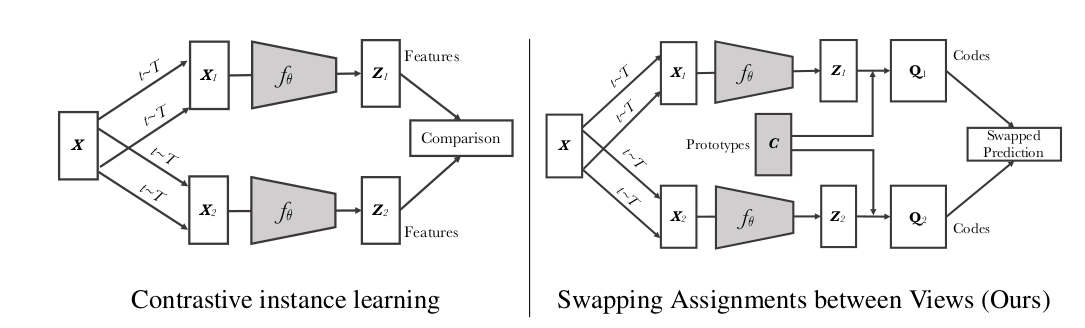
\includegraphics[scale=0.35]{images/swav.png}
        \caption{Visualization of SwAV \cite{caron_unsupervised_2021}}
    \end{center}
\end{figure}

\begin{figure}[h!]
    \begin{center}
        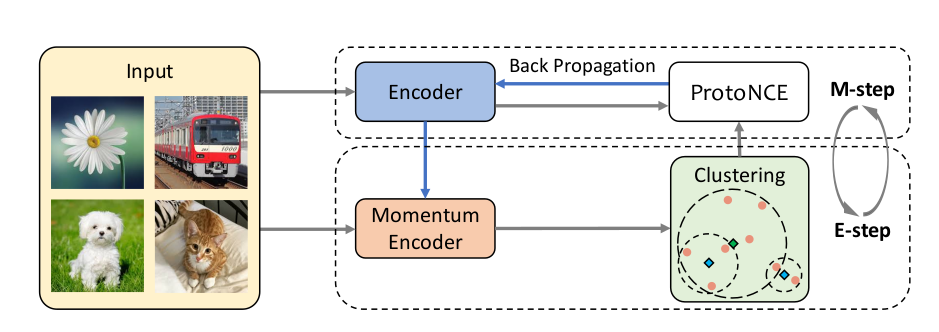
\includegraphics[scale=0.35]{images/prototypes.png}
        \caption{Visualization of PCL training framework \cite{li_prototypical_2021}}
    \end{center}
\end{figure}

\begin{figure}[h!]
    \begin{center}
        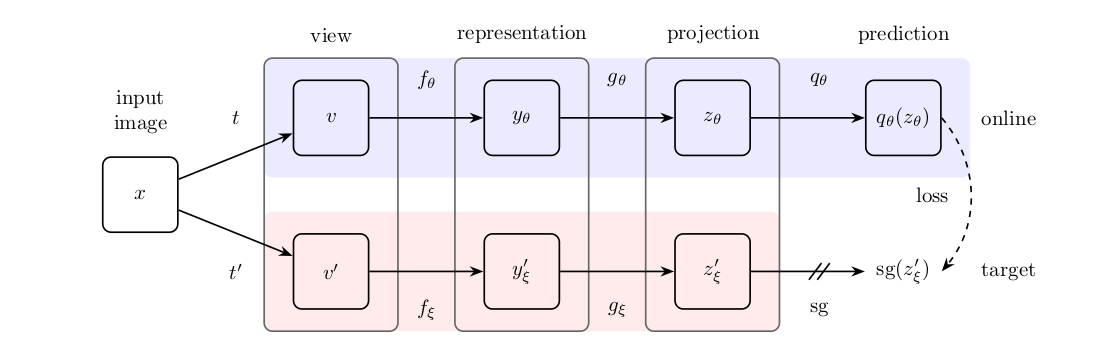
\includegraphics[scale=0.35]{images/byol.png}
        \caption{Visualization of BYOL \cite{grill_bootstrap_nodate}}
    \end{center}
\end{figure}

\subsection{Memory Banks \& Momentum Encoders}
\label{limitations:memory}

This method tries to deal with negative sampling by just having a lot of negative samples. This is obviously very brute force and requires a lot of compute resources. If we define $Q$ as a memory bank of fixed size that holds features from the previous iterations then we can reformulate the loss as:

$$\mathcal{L}_{i} = -\log \frac{\exp(q_{i} \cdot k^{+}_{i} / \tau)}{\exp(q_{i} \cdot k^{+}_{i} / \tau) + \sum_{k^{-} \in Q} \exp(q_{i} \cdot k^{-} / \tau)}$$

\subsection{Hard Negative \& Positive Mining}
\label{limitations:mining}

In the beginning when many negative samples are close to the query point, the gradient contribution from each negative sample is strong. But as training goes on, negative points become farther from the query and thus contribute much less to the gradient. Instead of tackling this using extremely large memory banks or batch sizes, this area of research tries to smartly select samples that best benefit encoder training and thus reduce the computational resources required and decrease the training time.
%

One approach is instead of using real data points, to generate synthetic data points from those negative samples that are closest to the query as was done in Mixing of Hard Negatives (MoChi) \cite{kalantidis_hard_nodate}. This creates more hard negative samples to train from and should increase the gradient contribution from the samples.
%

We can define these synthetic negatives as a mix of other negative samples that are most similar to the query point.

$$\mathbf{h}_k = \frac{\mathbf{h}_k}{\lVert \mathbf{h}_k \lVert^{2}}, \quad \text{where} \: \mathbf{h}_k = \alpha \mathbf{k_i} + (1-\alpha) \mathbf{k_j}$$

where $k_i$ and $k_j$ are randomly chosen from a set $\tilde{Q}$ of the logits that are most similar to the query point. Alpha is a mixing factor that is randomly selected from $(0,1)$. In theory, this shouldn't generate samples that are any harder than the existing negative samples but it does stretch the space around the query point more uniformly.

One way to make the task even harder is to mix the negative with the query point.

$$\mathbf{h}_k = \frac{\mathbf{h}_k}{\lVert \mathbf{h}_k \lVert^{2}}, \quad \text{where} \: \mathbf{h}_k = \beta \mathbf{q} + (1-\beta) \mathbf{k_i}$$

This technique however does not address the case where there may exist a large number of false negatives that would and should cluster around the query point.

Another approach that addresses this limitation is to remove these points from the dataset. Selecting false negatives is refereed to as a sampling bias in \cite{chuang_debiased_2020}. The key idea behind their approach is to approximate the underlying distribution of negative samples. They do this by accounting for the presence of positive samples in the denominator.

$$\mathcal{L}_{debiased} = -\log \frac{\exp(q_{i} \cdot k^{+}_{i} / \tau)}{\exp(q_{i} \cdot k^{+}_{i} / \tau) + Ng(x, \{u_i\}^N_i, \{v_i\}^M_i)}$$

$$g(x, \{u_i\}^N_i, \{v_i\}^M_i) = \frac{1}{\kappa^-}\max \{\frac{1}{N} \sum_i^N exp(q \cdot u_i)  - \tau^+\frac{1}{M} \sum_i^M exp(q \cdot v_i), \: \exp(\frac{1}{\tau})\}$$

where $\kappa^+$ is the uniform class probability and $\kappa^- = 1 - \kappa^+$
%

A followup work was presented in \cite{robinson_contrastive_2021}. They define informative negative samples as those that have embeddings close to the query but in reality should be far apart. They ask the question what makes a good negative point? Their answer is that 1) whose labels are different from the query point and 2) those whose embedding is most similar to the query point. They have a method to get the first principal approximately. The challenge is that points near the query are the hardest but also have a higher likelihood of being of the same class.

Their derivation is quite complicated but they end up with a similar formulation to \cite{chuang_debiased_2020} except with an additional parameter $\beta$ which specifies a concentration parameter. The formulation then becomes:

$$g(x, \{u_i\}^N_i, \{v_i\}^M_i) = \frac{1}{\kappa^-}\max \{ \eta \frac{1}{N} \sum_i^N exp(q \cdot u_i)  - \tau^+\frac{1}{M} \sum_i^M exp(q \cdot v_i), \: \exp(\frac{1}{\tau})\}$$

$$\eta = \frac{1}{N} \sum_i^N exp(\beta q \cdot u_i) $$

Not sure if this is right

Both of the above techniques \cite{chuang_debiased_2020} and \cite{robinson_contrastive_2021} have extremely simple implementations despite their complicated derivations.

It can be hard to tune properly
%

\begin{figure}[h!]
    \begin{center}
        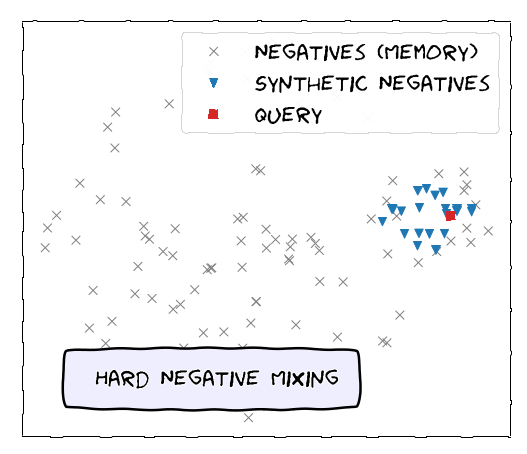
\includegraphics[scale=0.35]{images/synthetic-negatives.png}
        \caption{Negative Hard Mixing \cite{kalantidis_hard_nodate}}
    \end{center}
\end{figure}

\begin{figure}[h!]
    \begin{center}
        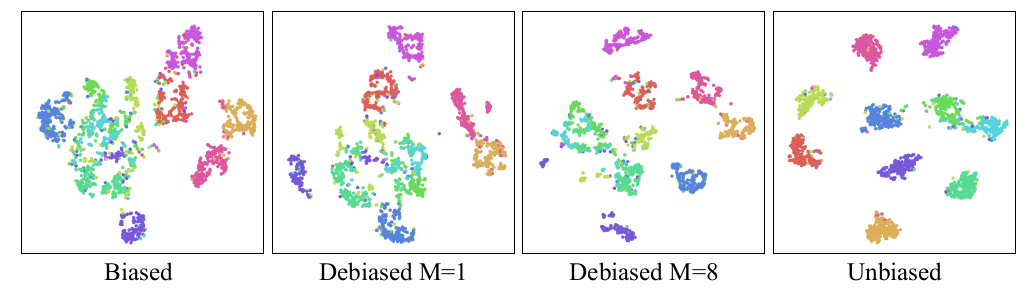
\includegraphics[scale=0.45]{images/debiased.png}
        \caption{t-SNE visualization of debiased objective \cite{chuang_debiased_2020}}
    \end{center}
\end{figure}
\newpage
\begin{figure}[h!]
    \begin{center}
        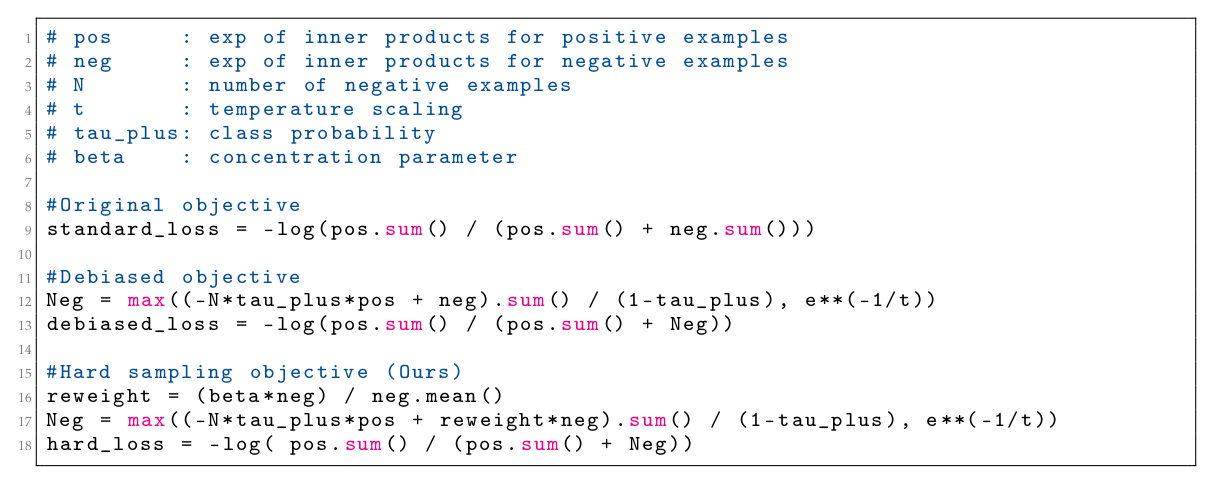
\includegraphics[scale=0.4]{images/hard-samplign.png}
        \caption{Pytorch pseudo code of hard sampling objectives. \cite{robinson_contrastive_2021}}
    \end{center}
\end{figure}

\newpage
\pagebreak
\newpage

\section{Proposal}

My work is focused on improving self-supervised contrastive learning in 3D point clouds for semantic and instance segmentation. I will use the work of PointContrast as my starting point. My focus will be on improving the Positive and Negative sampling strategies so that the pretext task and downstream performance improves as well as requiring fewer computational resources.

\subsection{Contrastive Loss}

It's been shown that InfoNCE loss with a temperature parameter is the most effective contrastive loss and the main one used in all recent vision applications. For this reason I will stick with this loss function. It is reprinted below for completeness.

$$\mathcal{L}_{i} = -\log \frac{\exp(q_{i} \cdot k^{+}_{i} / \tau)}{\exp(q_{i} \cdot k^{+}_{i} / \tau) + \sum^{K}_{j}\exp(q_{i} \cdot k^{-}_{j} / \tau)}$$

\subsection{Negative Sampling}

The main focus will be on improving the negative sampling techniques. Currently, negative samples are selected uniformly at random from the set of positive keys. However, this is a naive sampling strategy that is not conditioned on the sampled query point at all. It introduces the possibility for a large number of false negatives or semi-false negatives. Ideally we want to sample from a distribution like:

$$\mathbf{x}^{-} \sim p^{-}( \cdot | \mathbf{x})$$

To condition on the input point, I plan to use Fast Histogram Point Features (FHPF) as a way to select negative points that are sufficiently different from the input point. This operates on the assumption that if the point is different locally, then it for sure is different globally even if the surrounding area is the same.

$$p^{-}( \cdot | \mathbf{x}) = \text{Uniform}(\{ \: \mathbf{x}^- \: | \: \text{sim}(\text{FPFH}(\mathbf{x}^-),\text{FPFH}(\mathbf{x})) > \delta \})$$

where $\text{sim}(\cdot,\cdot)$ is some kind of distance function between the histograms such as earth movers distance.

\begin{figure}[h!]
    \begin{center}
        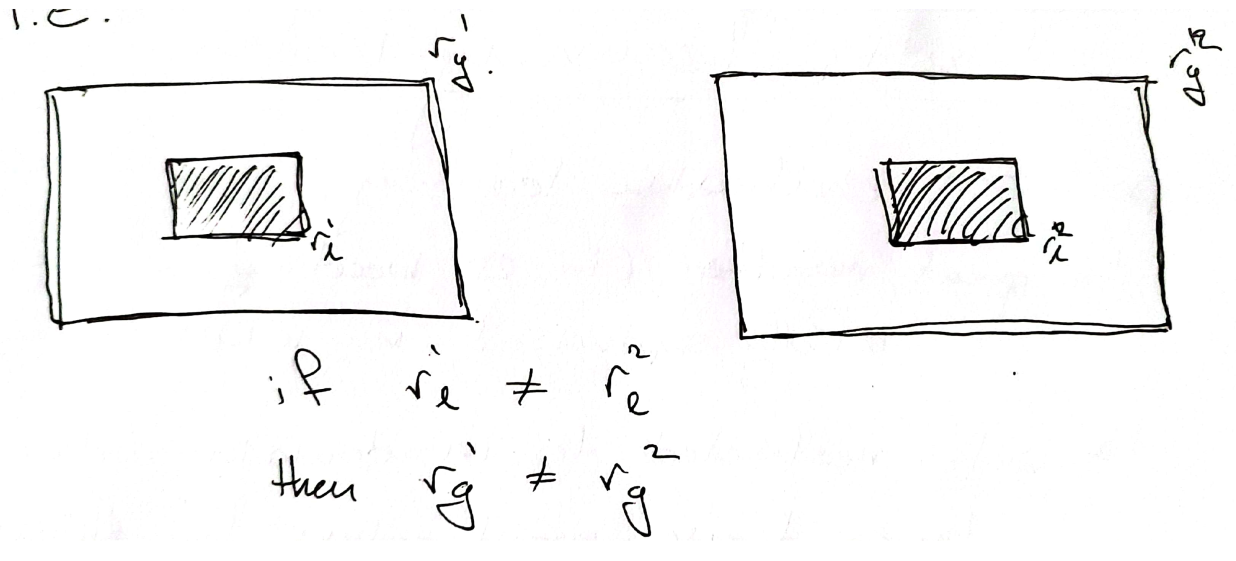
\includegraphics[scale=0.3]{images/regions.png}
        \caption{Visualization of local vs global region dissimilarity}
    \end{center}
\end{figure}

Instead of uniform sampling, I can also try cluster sampling by clustering different local features into feature types (e.g. flat surfaces, round objects, corners) and sample equally from those distributions.

$$p^{-}( \cdot | \mathbf{x}) = \text{Uniform}(\{ \textbf{c} \: | \: \textbf{c} \in \text{KNN}\{ \text{FPFH} ( \{ \: \textbf{x}^- \: | \: \textbf{x}^- \in \mathcal{X} \: \} ) \}, \textbf{c} \neq \textbf{x} \})$$

Where $\text{KNN}$ represents the K-nearest-neigbours clustering algorithm and $\textbf{c}$ is a set of negative samples clustered together based on their similar properties. Thus this strategy constitutes sampling equally from different clusters of points.
%

Another option is to weight the negative samples based off of the local dissimilarity of the points and incorporate this into the loss function itself.
%

$$\mathcal{L}_{i} = -\log \frac{\exp(q_{i} \cdot k^{+}_{i} / \tau)}{\exp(q_{i} \cdot k^{+}_{i} / \tau) + \sum^{K}_{j}\exp(w_{i,j} (q_{i} \cdot k^{-}_{j}) / \tau)}$$

$$\text{where} \: w_{i,j} = 1 - \frac{s_{i,j}}{\sum_k^{K}s_{i,k}} $$
$$ s_{i,j} = \text{sim}(\text{FPFH}(q_{i}), \text{FPFH}(k^{-}_{j}))$$

\begin{figure}[h!]
    \begin{center}
        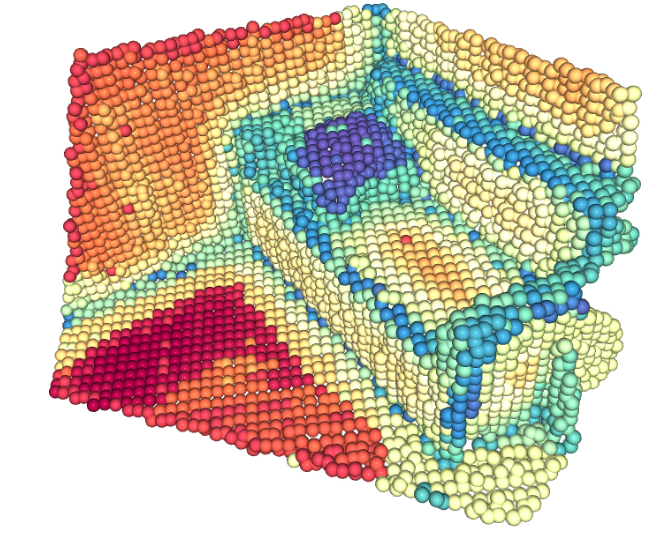
\includegraphics[scale=0.5]{images/fpfh.png}
        \caption{Visualization of Fast Point Feature Histogram features in a sample point cloud}
    \end{center}
\end{figure}

The last possibility is to look at applying different loss functions at different parts of the network depending on the receptive field. So that the parts looking at local regions have different objects than those looking at more global regions. Perhaps there's no advantage to training the global region at all?

\subsection{Positive Sampling}

The way you define positive sampling defines what you want the network to be invariant to. In the case where positive samples are different data augmentations, then the network will try to become invariant to these transforms. This may be desirable or undesirable for the task at hand. It has been shown in other works also that the positive sampling is what ultimately defines the hardness of the task.
%

Currently, the only data augmentations are random rotations. We can explore other kind of augmentations such as different elastic distortions but it may be too hard to learn as already it struggles to overfit. Another option is to train different networks to be invariant to different things such as one that is invariant to rotations and another that is not.
%

If we're using clusters, we can add points from the same cluster as other positive samples.
%

\subsection{Informative Sampling}

Beyond positive and negative sampling techniques, it maybe be beneficial to sample points that have locally interesting features. Currently many of the points that are sampled are those on the wall which is not very informative or helpful to the algorithm. During supervised training its able to learn walls and floors the quickest and with high accuracy so any pre-training for flat surfaces may be a waste of time.

Instead, we can to to select points according to the entropy of their feature vector.

$$p^{-}( \cdot | \mathbf{x}) = \text{Weighted}(\{ \: (w_i, \mathbf{x}^-_i) \: | \: \mathbf{x}^-_i \in \mathcal{X} \: \})$$

$$\text{where} \: w_i = \frac{\text{Entropy}(\text{FPFH}(\mathbf{x}^-_i))}{\sum_k^K \text{Entropy}(\text{FPFH}(\mathbf{x}^-_k))}$$

With $w_i$ being the weighted probability of the sample being selected.


\subsection{Other Techniques}

Although there does not exist and other kind of point sampling strategy in 3D (or even for 2D in fact), I would like to compare some of the other techniques that try to deal with the sampling problem.
%

I would like to compare my approach to one of each of the different options for addressing sampling issues. These being:

\begin{itemize}
    \item Momentum encoder from section \ref{limitations:memory}
    \item Hard negative sampling from section \ref{limitations:mining}
    \item Hard negative mixing from section \ref{limitations:mining}
    \item Clustering using either SwAV or BYOL from section \ref{limitations:clustering}
    \item Supervised contrastive from section \ref{limitations:supervised}
\end{itemize}

\pagebreak

\section{Results}

\subsection{Experimental Setup}

hyper-parameters:

\begin{itemize}
    \item batch size: 6
    \item accumulate gradient: 8
    \item learning rate: 0.2
    \item iterations: 4000
\end{itemize}

\subsection{Semantic Segmentation Pretraining}

\begin{center}
    \begin{table}[h!]
        \resizebox{\textwidth}{!}{
            \begin{tabular}{ c | c c c c c c c c c c c c c | c }
                                                                & ceiling        & floor          & wall           & beam           & column         & window         & door           & table          & chair          & sofa           & bookcase       & board          & clutter        & mIOU           \\
                \hline
                Baseline \cite{choy20194d}                      & 0.862          & 0.947          & 0.811          & \textbf{0.002} & \textbf{0.356} & 0.551          & 0.590          & 0.745          & 0.751          & 0.452          & 0.719          & 0.606          & 0.514          & 0.608          \\
                PointContrast \cite{xie2020pointcontrast}       & \textbf{0.905} & \textbf{0.962} & \textbf{0.818} & 0              & 0.345          & \textbf{0.581} & \textbf{0.633} & \textbf{0.750} & \textbf{0.861} & \textbf{0.648} & \textbf{0.729} & \textbf{0.799} & \textbf{0.566} & \textbf{0.661} \\
                \hline
                Entropy                                         & \textbf{0.912} & 0.961          & \textbf{0.828} & 0              & 0.307          & 0.513          & 0.626          & 0.746          & 0.853          & 0.634          & \textbf{0.742} & 0.761          & \textbf{0.576} & 0.651          \\
                Delta                                           & \textbf{0.924} & 0.959          & 0.817          & 0              & \textbf{0.388} & \textbf{0.611} & 0.563          & \textbf{0.770} & \textbf{0.867} & \textbf{0.667} & \textbf{0.742} & 0.635          & \textbf{0.587} & 0.656          \\
                Custer                                          & \textbf{0.924} & 0.957          & 0.814          & 0              & \textbf{0.373} & 0.562          & \textbf{0.688} & \textbf{0.776} & 0.844          & 0.524          & 0.729          & 0.717          & 0.587          & 0.653          \\
                \hline
                Debiased \cite{chuang_debiased_2020}            & 0.910          & 0.958          & 0.811          & \textbf{0.001} & 0.260          & 0.537          & 0.655          & 0.745          & 0.859          & 0.555          & 0.699          & 0.770          & 0.562          & 0.640          \\
                Debiased++ \cite{robinson_contrastive_2021}     & 0.901          & 0.961          & 0.815          & \textbf{0.008} & 0.286          & 0.586          & 0.683          & 0.745          & 0.855          & 0.599          & 0.716          & 0.779          & 0.554          & 0.653          \\
                \hline
                Sampling - Hard                                 & 0.904          & 0.959          & 0.824          & 0              & 0.361          & 0.579          & 0.659          & 0.731          & 0.837          & 0.505          & 0.697          & 0.711          & 0.557          & 0.640          \\
                Sampling - Easy                                 & 0.666          & 0.952          & 0.779          & 0              & 0.201          & 0              & 0              & 0.740          & 0              & 0              & 0.690          & 0.784          & 0.526          & 0.411          \\
                Sampling - Mixing \cite{kalantidis_hard_nodate} & 0.895          & 0.962          & \textbf{0.820} & 0              & 0.277          & 0.576          & \textbf{0.706} & 0.747          & 0.849          & 0.567          & 0.724          & 0.769          & 0.562          & 0.650          \\
                \hline
                Moco \cite{he_momentum_2020}                    & 0.888          & 0.941          & \textbf{0.831} & \textbf{0.001} & \textbf{0.369} & \textbf{0.582} & 0.610          & \textbf{0.752} & \textbf{0.863} & 0.578          & \textbf{0.749} & 0.758          & 0.565          & 0.653          \\
                BYOL \cite{grill_bootstrap_nodate}              & \textbf{0.907} & 0.958          & \textbf{8.25}  & 0              & 0.291          & 0.523          & \textbf{0.644} & 0.719          & 0.809          & 0.464          & \textbf{0.740} & 0.733          & 0.525          & 0.626          \\
                \hline
                CME - Encoder only                              & \textbf{0.911} & \textbf{0.963} & \textbf{0.818} & \textbf{0.002} & 0.278          & 0.541          & 0.521          & 0.733          & \textbf{0.883} & 0.524          & 0.705          & 0.756          & 0.559          & 0.630          \\
                CME - Full, SimSiam                             & 0.882          & 0.958          & 0.812          & 0              & 0.355          & 0.525          & 0.474          & \textbf{0.759} & \textbf{0.869} & 0.458          & 0.723          & 0.767          & 0.533          & 0.624          \\
                CME - Full, Contrast                            & 0.899          & 0.960          & 0.820          & 0              & 0.369          & 0.527          & 0.584          & 0.757          & 0.849          & 0.551          & 0.713          & 0.697          & 0.529          & 0.635          \\
            \end{tabular}
        }
        \caption{S3DIS pretraining results on Semantic Segmentation}
    \end{table}
\end{center}

\subsection{Experiment log}

\subsubsection{24.02.2022 - Image to 3D full pretraining}

\textbf{Details:} Ran 2D pre-training with SimSiam loss (which went to zero very quickly), then ran the same loss but between 2D to 3D using bi-linear interpolation to get the target feature vectors. Then finally ran full training on that.

\textbf{Results:} The error for 2D and 2D-3D went down way too quickly and became super small. However, on the final output of the pre-training it seems to have helped somewhat (0.608 to 0.624) but could certainly be better. Seeing as the embedding only got to 0.63 I think there's more performance to be had and it also validates the approach somewhat.

\subsubsection{25.02.2022 - Image Contrastive learning}

\textbf{Details:} Instead of using a BYOL loss with only positive samples, I went back to the old contrastive loss and was able to see a much more normal loss curve. Visualizing the results shows that it has learned key features in the images.

\textbf{Results:} Here are some sample visualizations:

\begin{figure}[h!]
    \begin{center}
        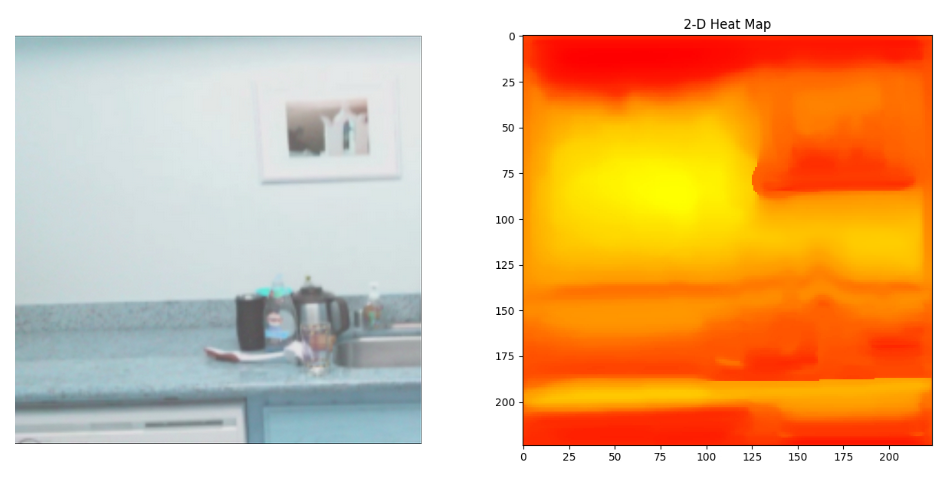
\includegraphics[scale=0.4]{images/experiments/25.02.2022-image-pretrain-vis1.png}
        % \caption{Visualization of pre-trained image features}
    \end{center}
\end{figure}

\begin{figure}[h!]
    \begin{center}
        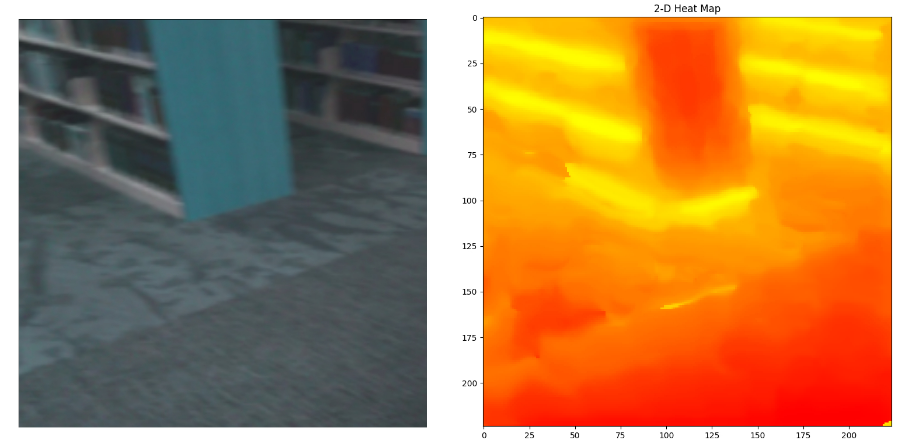
\includegraphics[scale=0.43]{images/experiments/25.02.2022-image-pretrain-vis2.png}
        % \caption{Visualization of pre-trained image features}
    \end{center}
\end{figure}

\begin{figure}[h!]
    \begin{center}
        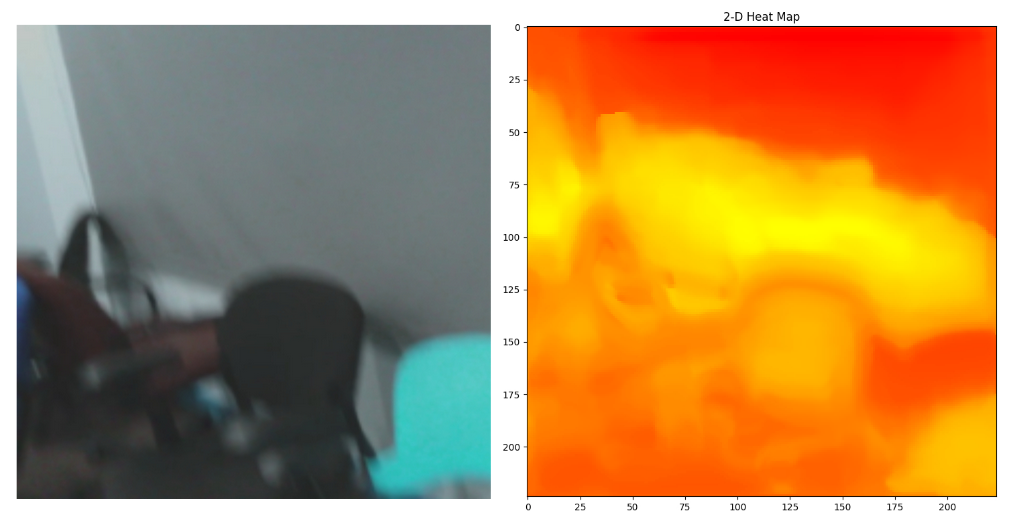
\includegraphics[scale=0.35]{images/experiments/25.02.2022-image-pretrain-vis3.png}
        % \caption{Visualization of pre-trained image features}
    \end{center}
\end{figure}

\subsubsection{01.03.2022 - Image to 3D full pretraining}

\textbf{Details:} Using the 2D Features learned from the previous experiment with a 2D pre-training objective, the goal was to transfer these 2D features over to the 3D points. This formed one side of the loss function, while the other side came from a 3D contrastive loss which compared points in the two transformed scans.

\textbf{Results:} The results seem to show an improvement over baseline, and slightly over previous attempts. So far the best effort from 2D transfer learning. But still much bellow PointGroup.

\newpage


\newpage
\bibliographystyle{plain}
\bibliography{contrastive-learning}

\end{document}